\documentclass{article}

\usepackage{graphicx}
\usepackage{tikz}
\usepackage{tikzsymbols}
\usetikzlibrary{calc,patterns,shapes.geometric}
\pagestyle{empty}
\usepackage[margin=0pt]{geometry}
\geometry{papersize={14in,12in}}

\def\centerarc[#1](#2)(#3:#4:#5){\draw[#1] ($(#2)+({#5*cos(#3)},{#5*sin(#3)})$) arc (#3:#4:#5);}

\begin{document}
	\begin{figure}
		\centering
		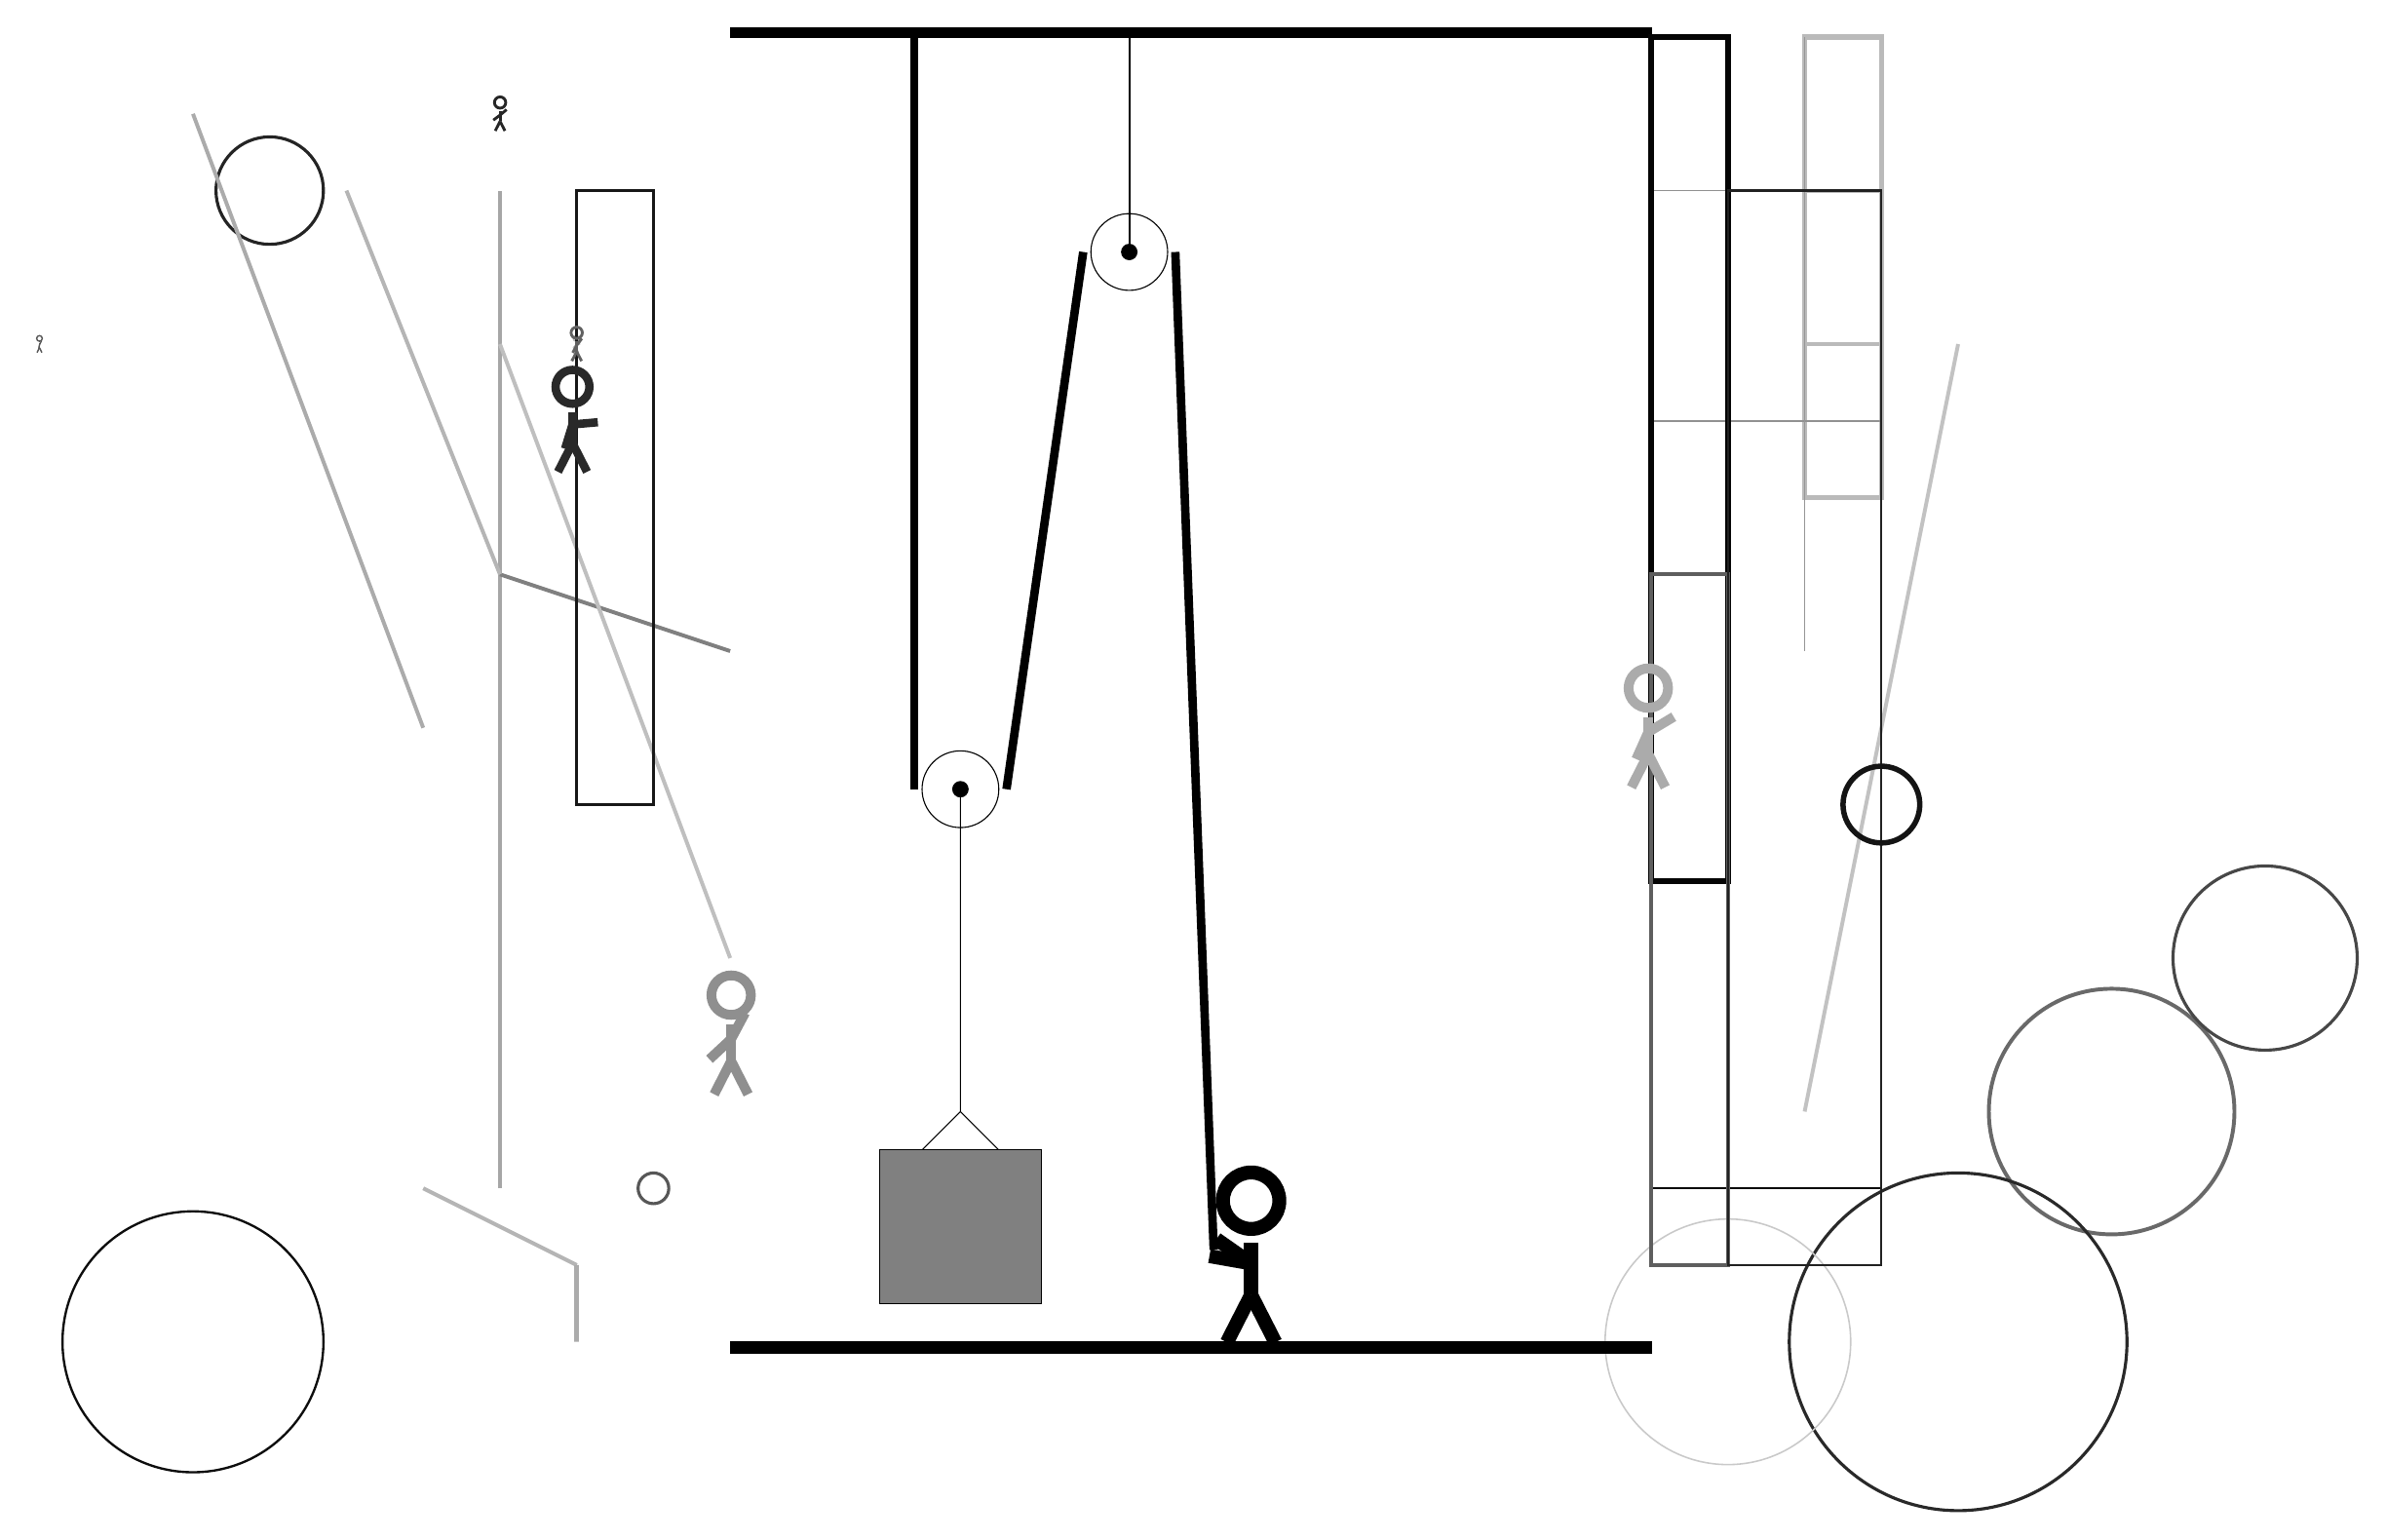
\begin{tikzpicture}
			%%%%% START %%%%%
			
			\draw[fill=black] (-2, 14) rectangle (10, 14.125);
			
			\draw (3.2, 11.2) circle (0.5);
			\draw[fill=black] (3.2, 11.2) circle (0.1);
			\draw[thick] (3.2, 11.2) -- (3.2, 14);
			
			\draw (1, 4.2) circle (0.5);
			\draw[fill=black] (1, 4.2) circle (0.1);
			
			\draw[line width=0.7mm, color=black!27] (12, 8) rectangle (13, 14);
			
			\draw [line width=0.4mm, color=black!86](-8, 12) circle (0.7);
			\draw[line width=0.5mm, color=black!27] (12, 10) rectangle (13, 12);
			\draw[line width=0.3mm, color=black!97] (10, -1) rectangle (13, -1);
			\draw [line width=0.5mm, color=black!59](16, 0) circle (1.6);
			\draw[line width=0.5mm, color=black!33](-6, 5) -- (-9, 13);
			\draw [line width=0.4mm, color=black!84](14, -3) circle (2.2);
			\draw[line width=0.5mm, color=black!29](-4, -2) -- (-6, -1);
			\draw[line width=0.3mm, color=black!66] (10, 1) rectangle (10, 6);
			\draw[line width=0.2mm, color=black!43] (10, 9) rectangle (13, 12);
			\node[line width=0.7mm, color=black!27] at (-4, 10) {\Strichmaxerl[1][47][10]};
			
			\draw [line width=0.4mm, color=black!66](-3, -1) circle (0.2);
			\draw[line width=0.5mm, color=black!35](-5, -1) -- (-5, 12);
			
			\draw[line width=0.2mm, color=black!41] (12, 6) rectangle (12, 14);
			\node[line width=0.7mm, color=black!44] at (-2, 1) {\Strichmaxerl[7][43][62]};
			\draw[line width=0.5mm, color=black!24](12, 0) -- (14, 10);
			
			\draw[line width=0.7mm, color=black!98] (11, 14) rectangle (10, 3);
			\draw[line width=0.5mm, color=black!50](-5, 7) -- (-2, 6);
			\node[line width=0.7mm, color=black!65] at (-11, 10) {\Strichmaxerl[1][80][62]};
			\draw [line width=0.2mm, color=black!21](11, -3) circle (1.6);
			\draw[line width=0.5mm, color=black!63] (10, 7) rectangle (11, -2);
			
			\draw [line width=0.3mm, color=black!95](-9, -3) circle (1.7);
			
			\draw[line width=0.5mm, color=black!25](-5, 10) -- (-2, 2);
			\draw[line width=0.4mm, color=black!91] (-4, 4) rectangle (-3, 12);
			\node[line width=0.7mm, color=black!62] at (-4, 10) {\Strichmaxerl[2][62][53]};
			
			\draw [line width=0.4mm, color=black!72](18, 2) circle (1.2);
			
			\draw[line width=0.3mm, color=black!87] (11, -2) rectangle (13, 12);
			\draw[line width=0.5mm, color=black!29](-7, 12) -- (-5, 7);
			\node[line width=0.2mm, color=black!85] at (-5, 13) {\Strichmaxerl[2][37][40]};
			\draw [line width=0.7mm, color=black!92](13, 4) circle (0.5);
			\draw[line width=0.6mm, color=black!33] (-4, -3) rectangle (-4, -2);
			
			\node[line width=0.3mm, color=black!84] at (-4, 9) {\Strichmaxerl[6][73][5]};
			\node[line width=0.6mm, color=black!33] at (10, 5) {\Strichmaxerl[7][66][31]};
			
			\draw (1, 4.2) -- (1, 0) -- (0.5, -0.5);
			\draw (1, 0) -- (1.5, -0.5);
			\draw[fill=black!50] (-0.05, -0.5) rectangle (2.05, -2.5);
			
			\draw[line width=1.1mm] (0.4, 14) -- (0.4, 4.2);
			\centerarc[line width=1.1mm](1, 4.2)(180:360:0.6);
			\draw[line width=1.1mm](1.6, 4.2) -- (2.6, 11.2);
			\centerarc[line width=1.1mm](3.2, 11.2)(0:180:0.6);
			\draw[line width=1.1mm](3.8, 11.2) -- (4.3, -1.8);
			
			\node at (4.7, -1.9) {\Strichmaxerl[10][-35][170]};
			
			\draw[fill=black] (-2, -3) rectangle (10, -3.15);
			
			%%%%% END %%%%%
		\end{tikzpicture}
	\end{figure}	
\end{document}